% Section: Lawvere: Logic Meets Category Theory

In the 1960s, F. William Lawvere showed that logic itself could be expressed categorically.

\begin{history}
Lawvere's thesis (1963) and subsequent work reformulated:
\begin{itemize}
    \item Theories as categories
    \item Models as functors
    \item Logical operations as categorical constructions (products, exponentials, etc.)
\end{itemize}
\end{history}

Let's unpack what this means.

\subsection{Conjunction is Product}

In logic, $A \land B$ is true when both $A$ and $B$ are true. To have evidence for $A \land B$, you need evidence for $A$ \emph{and} evidence for $B$.

In category theory, this is exactly a \textbf{product} $A \times B$: an object equipped with projections to both $A$ and $B$, universal among such objects.

\begin{center}
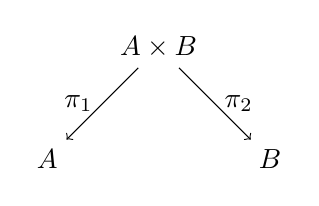
\begin{tikzpicture}[node distance=2cm]
    \node (AB) {$A \times B$};
    \node (A) [below left of=AB] {$A$};
    \node (B) [below right of=AB] {$B$};
    \draw[->] (AB) -- node[left] {$\pi_1$} (A);
    \draw[->] (AB) -- node[right] {$\pi_2$} (B);
\end{tikzpicture}
\end{center}

\textit{Having a proof of $A \land B$ means having a pair: a proof of $A$ and a proof of $B$.}

\subsection{Disjunction is Coproduct}

In logic, $A \lor B$ is true when at least one of $A$ or $B$ is true.

In category theory, this is a \textbf{coproduct} (or sum) $A + B$: an object with injections from both $A$ and $B$.

\textit{A proof of $A \lor B$ is either a proof of $A$ or a proof of $B$ (tagged with which one).}

\subsection{Implication is Exponential}

This is deeper. In logic, $A \to B$ means ``if $A$ then $B$.'' A proof of $A \to B$ is a \emph{method} that transforms any proof of $A$ into a proof of $B$.

In category theory, this is the \textbf{exponential object} $B^A$ (also written $[A, B]$ or $A \Rightarrow B$).

\begin{definition}[Exponential Object]
In a category, the \textbf{exponential} $B^A$ is an object representing ``morphisms from $A$ to $B$.'' It is characterized by a natural bijection:
\[
\mathrm{Hom}(C \times A, B) \;\cong\; \mathrm{Hom}(C, B^A)
\]
\end{definition}

What does this mean? Let's translate:

\textbf{Left side:} Maps from $C \times A$ to $B$. These are functions that take a pair $(c, a)$ and produce a $b$.

\textbf{Right side:} Maps from $C$ to $B^A$. These are functions that take a $c$ and produce a ``function from $A$ to $B$.''

The bijection says: a function of two arguments is the same as a function that returns a function. This is \textbf{currying}!

\begin{example}[In $\mathbf{Set}$]
In the category of sets, $B^A$ is exactly the set of all functions from $A$ to $B$:
\[ B^A = \{ f : A \to B \} \]
The bijection is currying:
\[ f(c, a) = b \quad\longleftrightarrow\quad g(c) = (\lambda a.\, f(c, a)) \]
\end{example}

\textit{Why the notation $B^A$? Because $|B^A| = |B|^{|A|}$---if $B$ has $m$ elements and $A$ has $n$ elements, there are $m^n$ functions from $A$ to $B$.}

\subsection{Quantifiers are Adjoints}

Now for the deepest part: quantifiers as adjoints.

First, what is an \textbf{adjunction}? Informally, two functors $F$ and $G$ are adjoint if they're ``almost inverses'' in a specific sense:

\begin{definition}[Adjunction, informally]
$F : \mathcal{C} \to \mathcal{D}$ is \textbf{left adjoint} to $G : \mathcal{D} \to \mathcal{C}$ (written $F \dashv G$) if there's a natural bijection:
\[
\mathrm{Hom}_{\mathcal{D}}(F(A), B) \;\cong\; \mathrm{Hom}_{\mathcal{C}}(A, G(B))
\]
\end{definition}

\textit{``A map out of $F(A)$ is the same as a map into $G(B)$.'' $F$ and $G$ are two perspectives on the same relationship.}

Now, how do quantifiers fit in?

Consider a projection $\pi : A \times B \to A$ (forgetting the $B$ component). This induces a functor $\pi^* : \mathbf{Set}/A \to \mathbf{Set}/(A \times B)$ that pulls back predicates.

\begin{itemize}
    \item \textbf{Existential quantifier $\exists$} is the \textbf{left adjoint} to pullback.

    \textit{``There exists a $b$ such that $P(a, b)$'' collapses the $B$-dimension by asking ``is there at least one?''}

    \item \textbf{Universal quantifier $\forall$} is the \textbf{right adjoint} to pullback.

    \textit{``For all $b$, $P(a, b)$'' collapses the $B$-dimension by asking ``does it hold for every one?''}
\end{itemize}

\begin{intuition}
Why adjoints? Because $\exists$ and $\forall$ satisfy these bijections:

\textbf{For $\exists$:} To prove $(\exists b.\, P(a,b)) \to Q(a)$, it suffices to prove $P(a,b) \to Q(a)$ (for arbitrary $b$). If $Q$ holds whenever $P$ holds for any specific $b$, then $Q$ holds when $P$ holds for \emph{some} $b$.

\textbf{For $\forall$:} To prove $Q(a) \to (\forall b.\, P(a,b))$, you must prove $Q(a) \to P(a,b)$ for each $b$. If from $Q$ you can derive $P$ for any specific $b$, then from $Q$ you can derive $P$ for \emph{all} $b$.

These are exactly the adjunction bijections in disguise!
\end{intuition}

\begin{keyinsight}
The duality between $\exists$ (left adjoint) and $\forall$ (right adjoint) is not a coincidence---it's the same duality that appears throughout mathematics:
\begin{itemize}
    \item Free structures (left adjoint) vs. forgetful functors (right adjoint)
    \item Tensor product (left adjoint) vs. Hom (right adjoint)
    \item Image (left adjoint) vs. preimage (right adjoint)
\end{itemize}
Quantifiers are just another instance of this universal pattern.
\end{keyinsight}

This is not just a translation. It reveals the \textbf{structural essence} of logic, stripped of the accidents of set-theoretic encoding. Implication, conjunction, disjunction, quantification---all emerge from categorical structure.

\begin{intuition}
A topos is a ``universe of mathematics'' with its own internal logic. Different toposes can have different logics: classical, intuitionistic, or even more exotic.

This unified logic and geometry: a topos is both a geometric object (like a space) and a logical universe (where you can do mathematics).
\end{intuition}
